\chapter{Introduction}

Speech is the most important medium of conveying opinions and expressing feelings and thoughts. Human convert their thoughts into speech by using words, phrases and sentences for communicating with each other \cite{mumtaz2016break}. Speech in human is generated by the vibrations in vocal cords with the air passage. Text to speech (TTS) synthesis is the process of transformation of textual data into voice output. In this process, small speech units called phonemes are joined in proper order to generate speech signals \cite{khilari2015review}. Speech data is obtained by first recording natural speech with the help of some type of recording systems and is converted to digital form. The digital data is sampled and stored in computer, after that passed back to analog signals and is converted back to speech \cite{greene1986perception}.

TTS systems are becoming important as they can be used in machines to effectively transmit information to human using artificial speech as information exchange through computers has become the integral part of new era. Visually impaired people usually suffer while using computer technology when there is no assistant or
computer is not enough interactive which makes TTS systems necessity of modern life. These systems increase the degree to which blind people can interact with sighted people \cite{klatt1987review} and could boost up their hope to survive in this world gracefully \cite{aida2010main}. Many applications of speech synthesis are emerging such as machines that read for blinds, aids for handicaps, computers that interact with user through speech. For all these applications, a text to speech conversion system is used \cite{klatt1982klattalk}.

The TTS system comprises of two main stages. One is called Natural Language Processing (NLP) and
other is called Speech Synthesis (SS). This is shown in figure \ref{fig:Main stages of TTS system}.

\begin{figure}
  \centering
  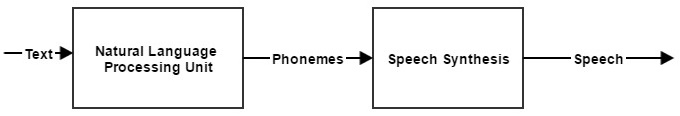
\includegraphics[width=\linewidth]{images/tts_bd.jpg}
  \caption{Main stages of TTS system}
  \label{fig:Main stages of TTS system}
\end{figure}

NLP unit is further divided in many sub processes. In start, word boundaries are marked by tokenizer which is called text normalization. This is followed by marking of syllable boundaries by using letter to sound rules. The syllabified data is processed to apply sound change rules. The data is also process to get context of each word in given sentence because for human, it is easy to guess context of each word in a sentence. For example, human can easily guess that if it is \texturdu{پل} (moment) or \texturdu{پل} (bridge) by reading a sentence. A computer program cannot guess that without context of that word. In the end, intonation and stress are added in the processed data. This processed data is then used in speech synthesizer to generate speech using different Digital Signal Processing techniques. The naturalness and intelligibility of the system is used to evaluate quality of the speech synthesizer.

In digital world, there are some people who can read and understand different languages and some who can’t understand languages except their own language. Speech to text conversion system can also provide a facility to exchange information between people speaking different languages \cite{khilari2015review}. TTS systems are also needed to reduce the extinction of minority languages. As minority languages of the world are facing challenge of extinction considerable efforts are going on from last few years for their survival. Fon language is spoken in Republic of Benin and some other regions of Africa and it is also facing challenge of extinction \cite{dagba2014text}. Similarly, the Xitsonga is the language which is spoken by the people of excess of three African nations. TTS system of such languages will help lot of people of different literacy level \cite{baloyi2012text}. Urdu is being spoken by more 70 million individuals on the planet \cite{top_30_languages} and it is national language of Pakistan and numerous states in India. A TTS system for Urdu will be extremely helping for partially or completely blind and illiterate people in these countries.

\section{Types of speech synthesis}
Different techniques exist for synthesizing artificial speech. Some of these techniques are discussed below.

\subsection{Formant synthesis}
In this technique, speech waveform is generated using concatenation of sine wave with the help of some algorithms to model a source of sound \cite{format_synthesis}. All speech parameters are changed periodically in order to get speech waveform. Some set of rules are also used to generate speech due to which this technique is also called rule based speech synthesis. As it is exceptionally hard to precisely portray speech generation process in set of rules due to which speech generated by this technique is not very natural but intelligible.

\subsection{Concatenative synthesis}
In concatenative synthesis, small units are selected from carrier sentences which are joined to form speech of complete sentence. These small units are called phonemes. The pronunciation of a word is described using collection of such units. As for any language, number of such units are few, therefor this procedure is simple when contrasted with the formant synthesis. English have 44 such phonemes. Urdu on the other hand have 44 consonants, 7 long nasal vowels, 3 short vowels, 8 long vowels, and many diphthongs \cite{saleem2002urdu}. This synthesized speech in this technique has less distortion but it is not very natural. That is the reason the produced speech may not look like the contributor speaker in training database \cite{huang1996whistler}.

\subsection{Statistical parametric speech synthesis}
Statistical parametric speech synthesis is another approach which is have become very popular in most recent couple of years and it works better than concatenative technique \cite{merritt2013investigating}. This technique is used with HMM or model which are firmly related to HMM e.g. Deep Neural Networks (DNN). HMM based statistical parametric speech synthesis has gained popularity because of its ability to produces high quality speech automatically with parametric flexibility, less data and resources \cite{black2007statistical}.

\section{Quality of speech synthesis system}
Intelligibility and naturalness is the measure of quality of the synthesized speech \cite{swetha2013text}. There are lots of experimentation over naturalness of voice as a result of TTS systems. In today’s world, different segments are recorded and then concatenated for completing a message. A collection of speech words is collected and maintained in database by using a reader who reads large series of text. In these kind of systems, to maintain the consistency the speaker speaks in a single style and keep in mind the distance from microphone and other factors to avoid the inconsistency. This type of TTS system is not required at all as the need is to have a system which can be expressive and convey message with proper expressions and styles. Work is performed to build a system that can convey the message according to the needs of the users. A single style of communication can lead towards wrong messages and can cause other problems of misunderstandings. For example, it is not appropriate to convey a good news and bad news in a same style and manner. Similarly, it is not acceptable to ask a question in neutral way of communication \cite{eide2004corpus}. Numerous strategies like neural networks and linear regression were applied to get the enhanced outcomes. Concatenation techniques are applied to get fully expressive and stylish messages for end users. By using concatenation technique, users can customize, add styles and expression through provided Speech Synthesis Markup Language (SSML) \cite{eide2004corpus}. In speech, Timing at which certain event occurs is also very important as in speech signals, it is affected by some contextual factors like phone identity factors. These factors make it difficult to control timing of events \cite{tokuda2000speech}. There are some approaches which have been proposed to control timing of events like linear regression \cite{kaiki1992linguistic} and tree regression \cite{riley1992tree}. A new technique is proposed in \cite{tokuda2000speech} where timing of events is controlled by multi-dimensional Gaussian distribution based Hidden Markov model.

\section{Architecture}
TTS system is a way of communication and transferring information using words and styles of speaking \cite{eide2004corpus}. It has two processes which are text processing and speech generation. In text processing, the given input text is processed so that to get appropriate chain of phonemic units. Speech generator takes these units as input and converts them into synthetic speech by selection of a unit from large corpus TTS system for small database is easier to implement but not in good quality \cite{black2007statistical, zen2007hmm, raj2007text}. Different researchers and developers used different strategies and architecture to develop TTS system. In \cite{kabir2002natural}, raw text is converted into intelligible speech signals by following two sub processes called High-level and Low-level synthesis. High-level synthesis converts textual data into phonetic strings and Low-level synthesis converts these strings into speech signals \cite{kabir2002natural}. In \cite{hussain2005phonological}, TTS system is divided into three modules.

\begin{enumerate}
  \item Natural language processing (NLP)
  \item Text parameterization
  \item Speech synthesis
\end{enumerate}

NLP unit converts text into phonetic strings. The second and third stages use these phonetic strings and convert them into speech signals. This is shown in figure \ref{fig:Architecture of TTS}.

\begin{figure}
  \centering
  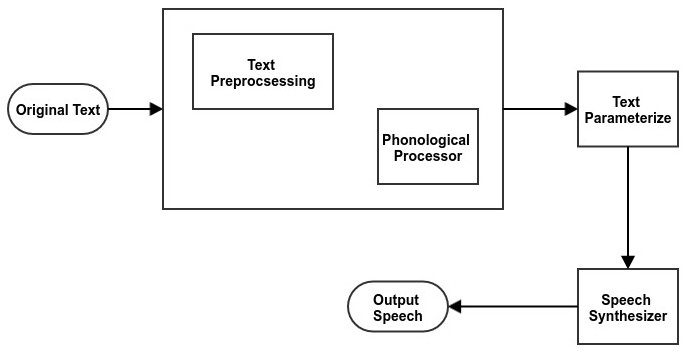
\includegraphics[width=\linewidth, height=7cm,keepaspectratio]{images/tts_block_dg.jpg}
  \caption{Architecture of TTS}
  \label{fig:Architecture of TTS}
\end{figure}
\\
In \cite{liberman1992text}, TTS system is implemented by following four modules in sequence.

\begin{enumerate}
  \item Text analysis
  \item Word pronunciation
  \item Phonetic interpretation
  \item Speech signal generation
\end{enumerate}

In text analysis, the input text is segmented into sentences and then divided into words. These words are then categorized according to their syntactic and contextual meaning. The numbers and abbreviations are also processed in this step. In word pronunciation process, words are represented by respective phonetic notations by using word pronunciation dictionary. In phonetic interpretation the duration of phonetic segments, pitch and accents are assigned. Signal generation component of TTS system takes output from all above processes and generate a signal of speech using a function. In \cite{urdu_text_preprocessing}, TTS system is divided in two parts. One is called NLP unit and other is called Speech Synthesis unit. NLP unit preprocess text and converts it into phonetic strings. These phonetic strings are then marked by stress marker and passed to speech synthesis unit which converts it into speech signals.
